\documentclass{bioinfo}
\copyrightyear{2014}
\pubyear{2014}


\usepackage{hyperref}



\begin{document}
\firstpage{1}

\title[PconsFold]{PconsFold: Improved contact predictions improve
 protein models}
\author[M.Michel \textit{et~al}]{Mirco Michel\,$^{1,2}$, Sikander
  Hayat\,$^{3}$, Marcin J. Skwark\,$^{4}$, Chris Sander\,$^{5}$, Debora
  S. Marks\,$^{3}$,  and Arne Elofsson\,$^{1,2,}$\footnote{To whom correspondence should be addressed.}}
\address{$^{1}$Department of Biochemistry and Biophysics, Stockholm University, 10691 Stockholm, Sweden, 
$^{2}$Science for Life Laboratory, Box 1031, 17121 Solna, Sweden, 
$^{3}$Department of Systems Biology, Harvard Medical School, Boston, Massachusetts, USA, 
$^{4}$Department of Information and Computer Science, Aalto University, PO Box 15400, FI-00076 Aalto, Finland, and
$^{5}$Computational Biology Center, Memorial Sloan-Kettering Cancer Center, New York, New York, USA}

\history{Received on XXXXX; revised on XXXXX; accepted on XXXXX}

\editor{Associate Editor: XXXXXXX}

\maketitle

\begin{abstract}

\section{Motivation:}
\red{Recently is has been shown} that the quality of protein contact
prediction from evolutionary information can be improved significantly
if direct and indirect information is separated. \red{Given
  sufficiently large protein families the contact predictions} contain
sufficient information to predict the structure of many protein
\red{families}. However, since the first \red{studies contact
  prediction methods have improved}. Here, we ask how much the final
models are improved if improved contact predictions are used.


\section{Results:} \red{In a small benchmark of 12 proteins from} we
show that the TM-score of top ranked models are improved by on average
33\% \red{using Pcons-fold compared to the orginal version of EVfold}.
In a larger benchmark we find that the quality is improved with
15-30\% \red{when using PconsC in comparson to earlier contact
  prediction methods.  Further,} using Rosetta instead of CNS does not
significantly improve global model accuracy \red{but} the chemistry of
models generated with Rosetta is improved.

\section{Availability:}
PconsFold is a fully automated pipeline for ab-initio protein
structure prediction based on evolutionary information. PconsFold is
based on PconsC contact prediction and uses the Rosetta folding
protocol. Due to its modularity, the contact prediction tool can be
easily exchanged. The source code of PconsFold is available on GitHub
at \url{https://www.github.com/ElofssonLab/pcons-fold} under the MIT
license. PconsC is available from \url{http://c.pcons.net/}.
\section{Contact:} \href{arne@bioinfo.se}{arne@bioinfo.se}
\section{Supplementary information:} Supplementary data are available at \emph{Bioinformatics} online.
\end{abstract}

\section{Introduction}
\begin{figure}[!tpb]%figure1
\centerline{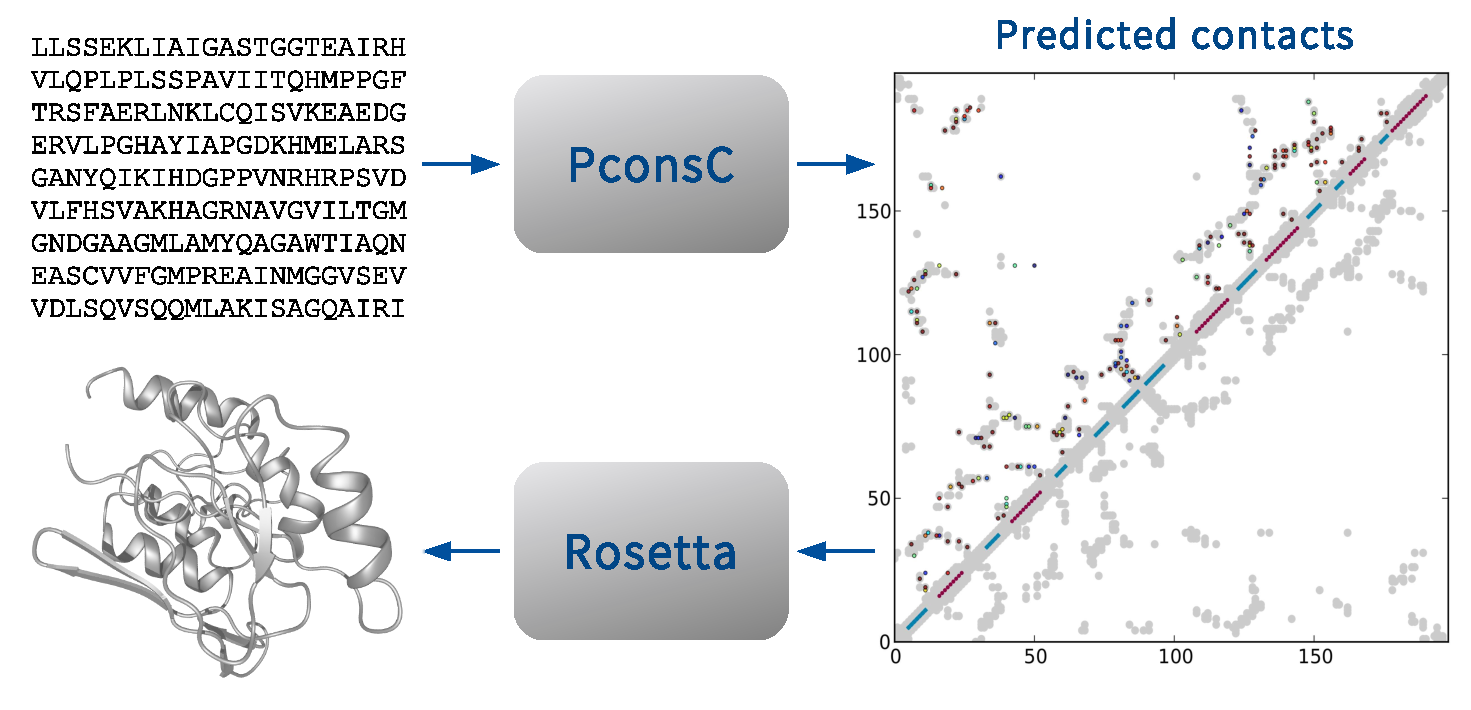
\includegraphics[scale=0.35]{figures/pipeline.eps}}
\caption{PconsFold pipeline. Based on a given protein sequence,
 amino-acid contacts are predicted with PconsC. These contacts then
 facilitate protein folding with Rosetta. In the end PconsFold
 outputs a structural model for the given
 sequence.}\label{fig:pipeline} 
\end{figure}

The protein folding problem is one of the
longest standing problems in structural biology. Although the problem
of physically folding up a single protein chain in the computer
remains largely unsolved, there have been continuous effort and
progress resulting in increased accuracy of predicted models
\cite[]{kryshtafovych_CASP10_2013}.

The idea of using residue-residue contacts predicted from analysis of
correlated mutations observed in evolution for 3D protein structure
prediction is not new
\cite[]{gobel_correlated_1994,Neher8278414,Hatrick16649265,Shindyalov_can_1994,Vendruscolo9377713}.
However, until recently contacts predicted from multiple sequence
alignments were not sufficiently accurate to facilitate structure
prediction methods significantly \cite[]{marks_protein_2012}.  This
only became possible due to a new statistical approaches to separate
direct from indirect contact information \cite[]{Lapedes1999,
  Lapedes2002, Weigt19116270,burger_disentangling_2010,
  morcos_direct-coupling_2011, marks_protein_2011} as well as a
greatly increased corpus of sequence information. These efforts came
to completion with the first demonstration of successful computation
of correct folds with explicit atomic coordinates using
maximum-entropy derived contacts \cite[]{marks_protein_2011}. Analysis
of the relative contribution of secondary structure and
co-evolutionary information pointed to potential improvements in 3D
accuracy \cite[]{Sulkowska22691493}. Since then there has also been
continuous effort to improve the quality of predicted contacts
\cite[]{jones_psicov:_2012, ekeberg_improved_2013,
  skwark_PconsC:_2013}.

In addition to the initial predictions of soluble proteins \cite[]{marks_protein_2011}
and protein-complexes \cite[]{Schug20018738}  contacts predicted from evolutionary information
have also been applied in structure prediction of membrane proteins
\cite[]{hopf_three-dimensional_2012, nugent_accurate_2012}.

To optimize protein structure prediction from predicted contacts we
developed PconsFold, a pipeline for ab-initio protein structure
prediction of  single-domain proteins, see Figure~\ref{fig:pipeline}. PconsFold is based on predicted
amino-acid contacts from PconsC. These contacts are utilized within
Rosetta to fold a given protein sequence from scratch. We benchmark
our method on two datasets and compare it to the CNS~\cite[]{Brunger18007608} protocol used in EVfold
\cite[]{marks_protein_2011}. It was found that the improved quality of predicted contacts
by PconsC~\cite[]{skwark_PconsC:_2013} increases quality and
native-likeliness of predicted structures by about 33\% over 
EVfold and 16\% over EVfold-PLM, that is using the improved contact
predictions from plmDCA~\cite[]{ekeberg_improved_2013}.

\begin{methods}
\section{Methods}

\subsection{Datasets}
During the development of PconsFold we used the proteins from
\citeauthor{jones_psicov:_2012} \citeyear{jones_psicov:_2012} (PSICOV
dataset). The dataset consists of 150 single domain proteins with sequence
lengths between 52 and 266 amino acids. A list of all Protein Data
Bank (PDB) \cite[]{berman_protein_2000} and corresponding Uniprot
\cite[]{magrane_uniprot_2011} IDs are given in Supplementary Table
1. 


For each protein we chose to use the PDB seqres sequence as input and
not the atom sequence. This avoids internal gaps due to missing
residues in the crystal structure.  Uniprot sequences were not
directly used to avoid including mutations and other sequential
differences with the PDB sequences. This also allows direct
comparisons between predicted models and native PDB structures. 

CNS~\cite[]{Brunger18007608} did not produce any models for the
protein 1JBE, which was therefore excluded from all evaluations.
{\color{red}We assume this was due to the unknown amino acid at
position 75.}

As an additional comparison between PconsFold and EVfold we used the set
of 15 proteins as in \cite{marks_protein_2011}. PDB and Uniprot IDs and the sequences are given in
Supplementary Table 2. According to the Uniprot IDs we extracted the sequences from the
Pfam alignments that were used in the publication. These sequences were
submitted to the EVfold web-server and used as input for PconsFold.

\subsection{Contact prediction}
In PconsFold residue contacts are predicted using
PconsC \cite[]{skwark_PconsC:_2013}. The contact predictor
plmDCA \cite[]{ekeberg_improved_2013} is used by Rosetta/plmDCA and in
EVfold-PLM. Rosetta/plmDCA utilizes the direct output from plmDCA,
while in EVfold predicted contacts are further optimized according to
\cite{marks_protein_2011}. PSICOV \cite[]{jones_psicov:_2012} was used
in Rosetta/PSICOV.


Predicted contacts were ranked according to the confidence score
assigned by the respective contact prediction method. For each protein
we selected $n = f \cdot l$ top-ranked contacts, where $l$ represents
the length of the protein sequence and $f$ a factor to scale $n$
relative to sequence length. {\color{red} Consider $f$ is set to 1.0.
A protein with length 100 amino acids will thus be constrained by the
first 100 predicted contacts.}



\subsection{Rosetta}
In PconsFold, Rosetta/plmDCA, and Rosetta/PSICOV we apply the
AbinitioRelax folding protocol \cite[]{rohl_protein_2004} of Rosetta
in version 2013wk42 \cite[]{leaver-fay_rosetta3:_2011}. The file {\tt
 abinitio.options\_tmpl} in the folder {\tt pcons-fold/folding/rosetta} of the GitHub
repository lists all options we are using with AbinitioRelax. 

We employ the function \emph{FADE} to integrate predicted residue
contacts into the internal scoring function of Rosetta. \emph{FADE}
calculates the energy of a given contact as a function of the distance
$d$ between its residues as given by the following equation:

\begin{equation}%\label{eq:fade}
\textit{FADE}(d) = \left\{
\begin{array}{l l l}\label{eq:fade}
%2b_{low}^3 - 3b_{low}^2 + 1 & \quad \textrm{if d $<$ $c_{low}$} \\
%2b_{up}^3 - 3b_{up}^2 + 1 & \quad \textrm{if d $>$ $c_{up}$} \\
0.0 & \quad \textrm{for $d < lb$ or $d > ub$} \\
-2(\frac{d - \textit{lf}}{z})^3 - 3(\frac{d - \textit{lf}}{z})^2 + 1 & \quad \textrm{for $d < \textit{lf}$} \\
2(\frac{d - \textit{uf}}{z})^3 - 3(\frac{d - \textit{uf}}{z})^2 + 1 & \quad \textrm{for $d < \textit{uf}$} \\
w & \quad \textrm{otherwise.} \\
\end{array} \right.
\end{equation}

The parameters $lb$ and $ub$ are lower and upper bounds, $z$
represents the fading zone's width, $\textit{lf}$ and $\textit{uf}$
denote the inner boundaries for the fading zone $lb + z$ and $ub - z$,
respectively. The well depth of the interval between both inner
boundaries is given by $w$. We set $lb$ to -10 \AA, $ub$ to 19 \AA\
and $z$ to 10 \AA. This defines a contact to be fully formed if the
participating residues are within 9 \AA\ of each other. The fading
zones allow for a soft margin between formed and non-formed
contacts. In terms of energy all non-formed contacts are ignored. In
our opinion this accounts best for the fuzzy nature of predicted
contacts. The fading zone at the lower bound allows Rosetta to detect
and resolve overlapping residues, i.e. when there is a negative
distance between two residues. 


To avoid the inclusion of homologous fragments into Rosetta, the {\tt
  -nohoms} flag was used during fragment
picking. This means that only fragments from non-homologous protein structures were selected. This
was done to simulate a real application case and not to overestimate
prediction performance. If not stated otherwise, we used all 150 proteins of
the PSICOV dataset as prediction targets in this section. 


\subsection{Folding with CNS using EVfold-PLM}
On the PSICOV dataset EVfold-PLM was run in a standalone version. The
alignment E-value cutoff was fixed to $10^{-4}$. The parameter $m$ was
set to 0.9. This defines a threshold to exclude sequences from the
alignment that consist of more than 90\% of gaps. Using just one E-value for the alignment  enabled comparison across the methods but it should be noted that the EVfold server offers optimization of the E-values based on sequence coverage and number of sequences found, which results in improved results in some cases. 

EVfold-PLM was run with default parameters on the small test set using
the web-interface available at \url{http://evfold.org/}. We ensured
that it uses pseudolikelihood maximization (plm) on all data, instead of the na\"ive mean field approach for contact prediction.

Folding with EVfold-PLM was performed using CNS and the same protocol
as described before~\cite[]{marks_protein_2011}. Here, the distance
geometry protocol is initially used and followed by a short simulated
annealing. The CNS based {\color{red}folding} protocol used in EVfold is approximately
one order of magnitude faster than the Rosetta protocol used in
PconsFold. In addition PconsC is at least four times slower than just
running the contact predictions used in EVfold-PLM.

\begin{figure*}[!tpb]%figure1
\centerline{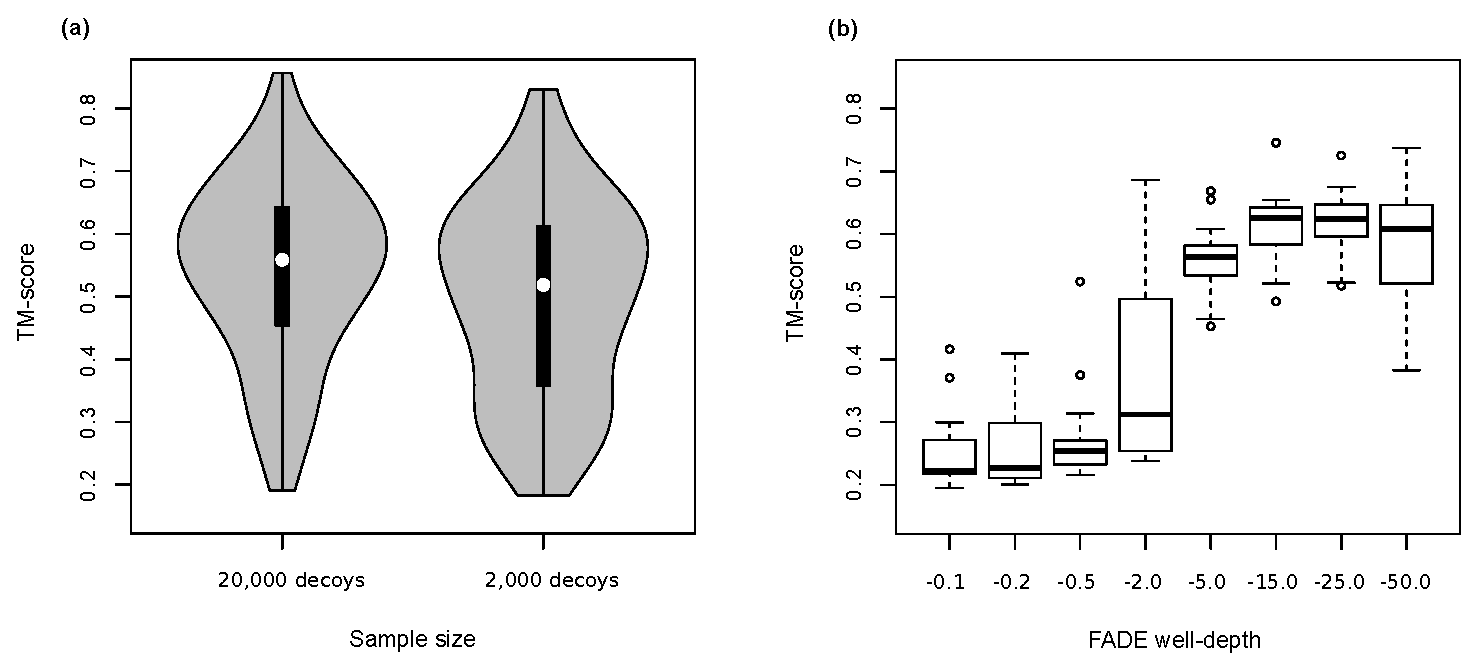
\includegraphics[scale=0.7]{figures/rosetta.eps}}
\caption{Model quality in TM-score for adjustments of two
 different Rosetta parameters. (a) Performance distributions 
 for two different sample sizes of 20,000 (left) and 2,000 (right) 
 decoy structures. The black boxes indicate upper and lower 
 quartile with white dots at the median of the distributions. For each 
 protein in the full PSICOV dataset the top 
 ranked model was selected from the decoys by its Rosetta score and 
 compared to the native structure. (b) Effects of adjustments to 
 the well-depth parameter of the FADE function. A low absolute 
 well-depth (left side) puts low weight on predicted constraints. 
 Constraints are stronger weighted by higher absolute values of 
 well-depth (right side). A subset of 14 proteins of the PSICOV dataset was used here.}\label{fig:ros} 
\end{figure*}



\subsection{Identification of top ranked model}

In addition to internal Rosetta scoring we assessed the quality of all
predicted models with the model quality assessment programs (MQAPs)
Pcons \cite[]{lundstrom_pcons:_2001}, ProQ2
\cite[]{ray_improved_2012}, and DOPE from the Modeller software
package \cite[]{eswar_comparative_2006}. Pcons uses a comparative
approach and ranks all decoys according to pairwise structural
similarity between them. ProQ2 and DOPE assess single proteins and
evaluate structural features, such as side-chain placement and overall
shape. For our ranking we use the global score each MQAP assigns to a
predicted structural model (decoy). Residue-wise information about
local model quality is thus not used. 

For each structure prediction method all decoys were re-ranked with
each MQAP. The top-ranked model was then selected and compared to its
native structure. For this comparison we used the TM-score
\cite[]{zhang_scoring_2004} as a measure of structural similarity. As
native structure we used the PDB structure of each protein without
further loop-closing or other refinement. Residues present in seqres
but not observed in the crystal stucture, although modeled, are therefore ignored in the structural
comparison.

The positive predictive value (PPV) was calculated to assess the
quality of predicted models. It indicates how well a given contact map
fits a given structure. All PPV values were calculated using reference
contacts C$^{\beta}$ (C$^{\alpha}$ in case of glycine) distances in
the structure (native or model) with a cutoff at 8 \AA.


\subsection{Model quality assessment}

We used MolProbity \cite[]{chen_molprobity:_2010} to assess the chemical
model quality. The MolProbity tool {\tt oneline-analysis} was used to 
detect clashes and to evaluate backbone dihedrals as well as 
side-chain rotamers. To prepare all structures for this analysis, we 
first relaxed them with fixed backbone atoms.
The Rosetta protocol {\tt relax.linuxgccrelease} was used with the flags 
{\tt -relax:quick} {\tt -in:file:fullatom} {\tt 
-constrain\_relax\_to\_start\_coords}. Hydrogen atoms were then 
added with the MolProbity tool {\tt reduce-build}. All resulting 
structures are provided in the Supplementary Material.



\subsection{Running time}
A reduction from 20,000 to 2,000 decoy structures corresponds to a 10-fold
decrease of runtime during the Rosetta folding step but also leads to an
expected decline in average model quality{\color{red}, see Figure~\ref{fig:ros}a}. On one core of an Intel
E5-2660 (2.2 GHz Sandybridge), the calculation of one decoy takes
between 1 and 10 minutes for the shortest and longest protein in the
PSICOV dataset respectively. To compute 2,000 decoys for each protein
we ran 16 threads in parallel. Each of these threads then generates
125 decoys, starting with independent random seeds. With this setting
it takes between two hours and nearly one day to generate all decoys
for one protein. This simple scaling is possible since Rosetta runs
are independent of each other as long as they are based on 
independent random seeds. Increasing the number of threads can then be used to reduce
overall runtime or to generate more decoys within a given timespan.

\end{methods}


\section{Results and Discussion}

\subsection{PconsFold}


For all results in this section, we used the internal Rosetta score to
rank all predicted decoys. The top-ranked decoy structure was then
selected as the  final model.

Previous studies have shown that 20,000 -- 200,000 decoys are
necessary to sample native-like conformations without using spatial
constraints \cite[]{Simons10526365}. We set out using 20,000 models
and then reduced the number of decoy structures to 2,000. The bulk at
around 0.3 TM-score observed for when only 2000 models are generated
represents an increased number of low quality models, see
Figure~\ref{fig:ros}a. In general the practical advantages of
massively shorter Rosetta runs outweigh slightly worse predicted
models. This parameter is therefore set to a default value of 2,000
but can be specified by the user via a command line argument. All
further results in this section are generated with this default
setting, ie. using 2000 models. 


We selected the FADE function to incorporate predicted residue
contacts into Rosetta's native energy function. We then optimized the
parameter $w$ (well-depth) of FADE (Equation~\ref{eq:fade}).
{\color{red}A subset of 14 proteins of the PSICOV dataset, see
Supplementary Table 1, was used to reduce CPU hours of this step.} The
resulting TM-scores are shown in Figure~\ref{fig:ros}(b). The energy
term from spatial constraints diminishes with well-depth values of
-0.5 and above. This leads to a significant decrease in model quality.
Stronger weights than -5.0  put a larger absolute weight on the
constraints resulting in higher model qualities. {\color{red} This
trend can also be observed when looking at the full dataset. The
average TM-score decreases to 0.28 using a well-depth of -1.0.} At the
end we choose to use a value of -15.0 to achieve high model quality
without outweighing Rosetta's internal energy function completely.


\begin{figure*}[!tpb]%figure1
\centerline{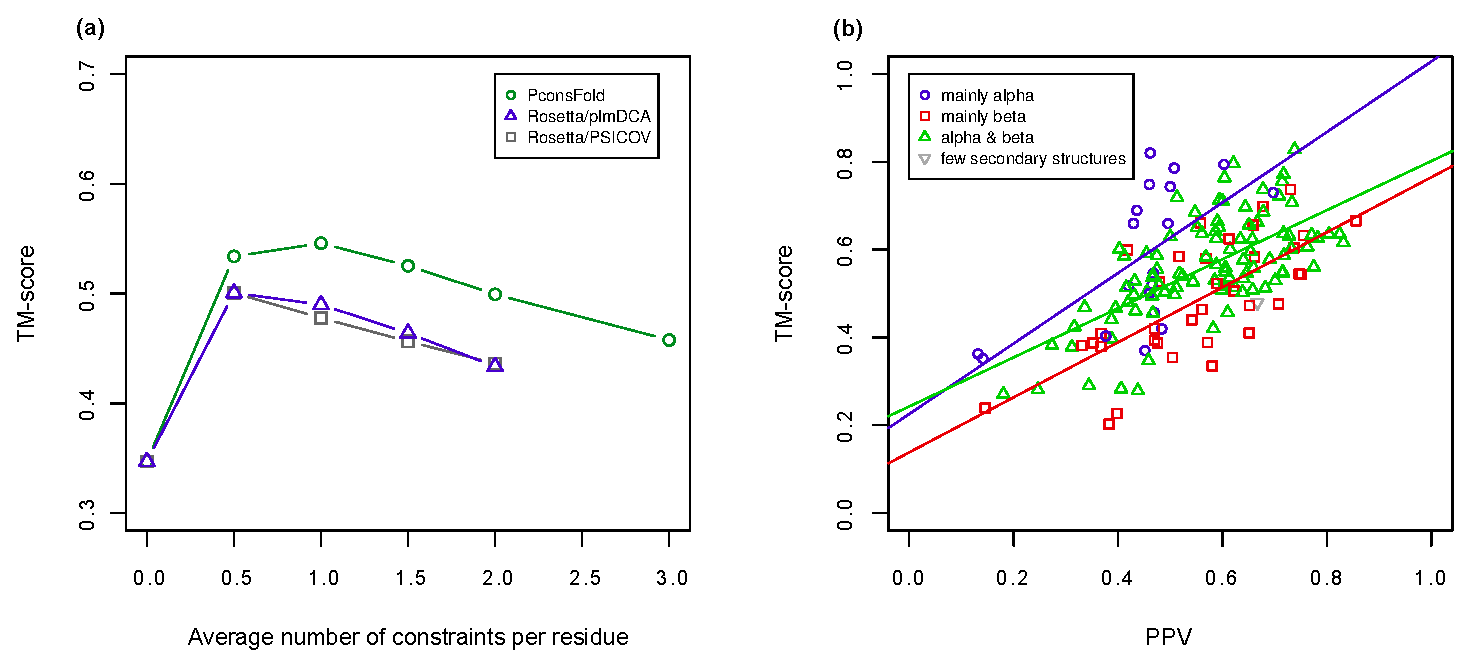
\includegraphics[scale=0.7]{figures/tmscores.eps}}
\caption{Folding performance on the full PSICOV dataset. (a) The 
 number of contacts used in structure prediction is
 plotted against average TM-score for three different methods:
 PconsFold (green circles), Rosetta/plmDCA (blue triangles), and
 Rosetta/PSICOV (black squares). For each protein the number of top
 ranked contacts was selected relative to its sequence length. A value
 of 1.0 on the $x$-axis represents one
 contact per residue on average. {\color{red}Error bars indicate
 standard errors.} b) TM-scores are compared
 to the PPV of underlying contact maps for PconsFold (using
 PconsC). The colors represent all four CATH fold classes. Lines 
 are fitted to the data to illustrate performance differences between the fold classes.}\label{fig:main}
\end{figure*}

With any number of contacts used during structure prediction, the
resulting model quality is on average higher than it would be without
contact information. Figure~\ref{fig:main}a shows that predicted contacts generally improve model
quality, regardless of method or amount of contacts. 


{\color{red}In addition, improvements in contact prediction methods further increase the quality
of predicted structures.} With an average TM-score of 0.55
PconsFold, i.e. using PconsC contacts provides a 10\% improvement
over using PSICOV or plmDCA contacts. This observation is consistent
with a direct comparison of contact prediction methods as in
\citeauthor{skwark_PconsC:_2013}
\citeyear{skwark_PconsC:_2013}. However, the performance difference
between PSICOV and plmDCA diminishes when their contacts are used in
structure prediction. 


There is an optimal number of contacts, specific to the contact
prediction method. In Figure~\ref{fig:main}a the average TM-score
maximum is reached at $x=1.0$ for PconsFold, while for PSICOV and
plmDCA fewer contacts provide better models. This can be explained by
the quality of predicted contacts, i.e. there exists a larger number of
correct contacts in PconsC compared to plmDCA or PSICOV \cite[]{skwark_PconsC:_2013}. Using more of these contacts during
structure prediction leads to improved models.


This relation between contact and model quality can also be observed
in Figure~\ref{fig:main}b. The overall Pearson correlation between PPV and TM-score in
this dataset is 0.59, i.e. proteins with contact maps of lower quality tend
to be modeled less accurate. 


Proteins belonging to the {\it mainly alpha} CATH fold class seem to
be easier to fold than proteins from the {\it alpha \& beta} fold
class and proteins from the {\it mainly beta} fold class seem to be
hardest to fold, see Figure~\ref{fig:main}. On average predicted contact maps in
mainly $\alpha$-helical proteins (blue) have similar or lower PPV
values than those of $\beta$-sheet containing proteins (green and
yellow), but the resulting models are more accurate in terms of
TM-score.




\subsection{Identification of top ranked model}

Table~\ref{tab:qa} summarizes the evaluation of different MQAPs on the
predictions for the PSICOV dataset. It shows average TM-scores for
top-ranked models after re-ranking all models with each MQAP.
{\color{red}Due to the different ways constraints are used within CNS
and Rosetta, we did not apply Rosetta's internal scoring function to
the models generated by CNS.} {\color{red}To provide a TM-score
baseline we ran the Rosetta folding step without constraints and
using the internal scoring only (Rosetta/baseline).} {\color{red}For
PconsFold and Rosetta/plmDCA the internal scoring performed best,
which is indicated by the highest average TM-score in
Table~\ref{tab:qa}.} The internal scoring function takes into account
the number of satisfied predicted contacts as a part of the energy
function, i.e. models that satisfy more predicted contacts are
assigned low energies and thus ranked on top.

In  EVfold-PLM the best method to identify top-ranked models is by
using Pcons~\cite[]{lundstrom_pcons:_2001}.
Further, Pcons performed only slightly worse than the internal scoring
function of Rosetta on the models from PconsFold and
Rosetta/plmDCA, showing the advantage of simple clustering methods.

Further, we examined two quality assessments that have been reported
to show good ability to identify accurate protein models, ProQ2~\cite[]{ray_improved_2012} and Dope~\cite[]{Shen17075131}.
The ProQ2 quality did not perform well on EVfold-PLM models but only slightly worse than
Pcons on models from PconsFold and Rosetta/plmDCA. We also tested a
combination of ProQ and Pcons, as in \cite{wallner_pcons.net:_2007}. However, the results are omitted
since they were not significantly different from those of Pcons
alone. DOPE scoring of EVfold-PLM models worked almost as good as Pcons,
but we observe a strong decline in average model quality for PconsFold
and Rosetta/plmDCA. 

\begin{table}[!t]
    \processtable{{\color{red}Average TM-scores for top-ranked models.
    Models were ranked by different MQAPs.} \label{tab:qa}}
{\begin{tabular}{lllll}\toprule
        Method & EVfold-PLM & Rosetta/plmDCA & PconsFold & Rosetta/baseline  \\ \midrule
        Rosetta & -- & 0.50 & 0.55 & 0.34 \\
        Pcons & 0.47 & 0.47 & 0.53 & -- \\
        ProQ2 & 0.36 & 0.46 & 0.51 & -- \\
        DOPE & 0.46 & 0.32 & 0.36 & -- \\ \botrule
\end{tabular}}{}
\end{table}

\begin{figure*}[!tpb]%figure1
\centerline{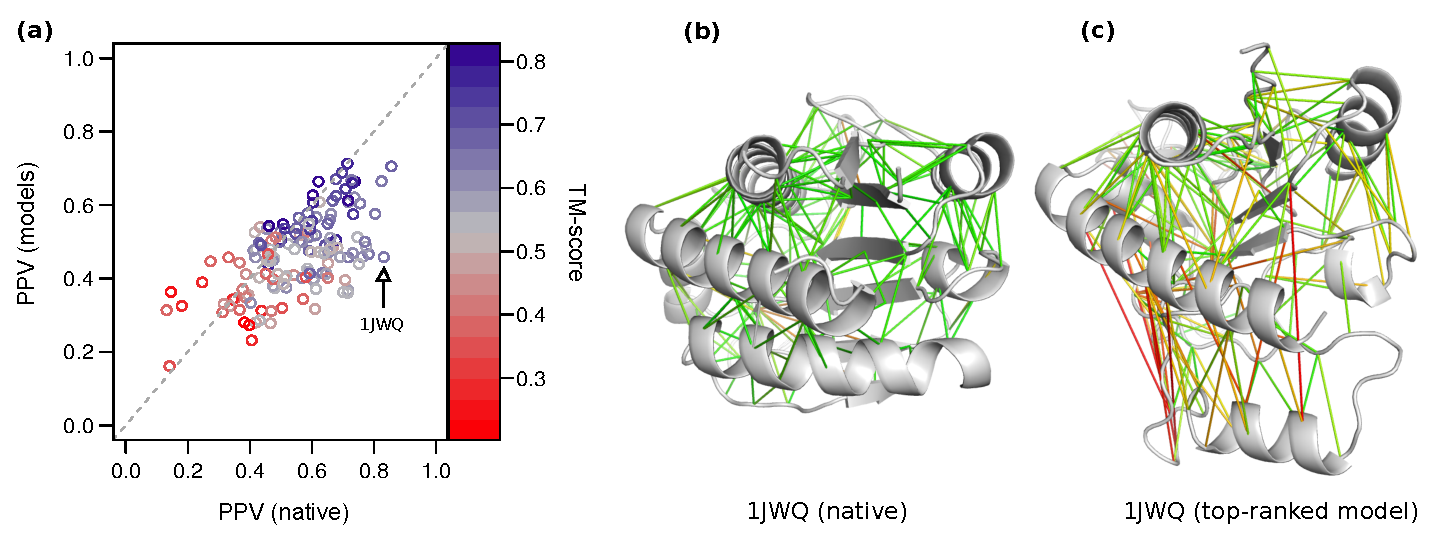
\includegraphics[scale=0.7]{figures/qa.eps}}
\caption{Analysis of contact maps in native structures and
top-ranked models. PPVs were calculated for the sets of contacts that
were used during folding ($1.0 \cdot l$ top-ranked contacts) with a
C$^\beta$ distance cutoff of 8~\AA\ in the structures. (a) PPV values for PconsC contacts on native structures 
($x$-axis) against PPVs on the top-ranked models from PconsFold 
($y$-axis). The colors represent TM-scores of models against native
structures. (b) Native structure of 1JWQ. Lines represent all predicted contacts. The color 
scheme indicates spatial distances of residue pairs in the 
structure. The PPV is 0.83. (c) Predicted contacts in the top-ranked 
model for 1JWQ with the same color scheme. This model has a TM-score 
of 0.62 and a PPV of 0.46}\label{fig:qa}
\end{figure*}

\subsection{Does PconsFold optimally use the contact information ? }

Next, we examined if the folding protocol has fully utilized the
available contact information. This was done, by comparing the number
of satisfied constrains (PPV) in the top ranked model and the native
structure.  On average the PPV of predicted contacts is higher in
native structures than in the models (0.55 vs. 0.47). This shows that
using a more efficient folding protocol would improve the models. All
points in the lower right triangle in Figure~\ref{fig:qa}a indicate
models that could be improved.  Clearly, for predicted contacts below
PPV=0.4 many models satisfy the constraints better than the native
structures, i.e. we would not expect that a better folding protocol
would improve the models.  It is possible that these low quality
contact maps mislead the structure prediction process and that this
results in models that diverge from native structures with a better
fit to the predicted contacts. Possibly, in these cases it would be
better to use fewer contacts. 
However, for most proteins with a PPV higher than 0.4 we are
clearly not able to satisfy all constraints. Here, an improved folding
protocol would improve the models.


In Figure~\ref{fig:qa} we also study one example of non-optimal
folding more closely. We selected 1JWQ since it represents the
worst-case scenario where the difference between native and model PPV
is largest. With a PPV of 0.83 most of the contacts were predicted
correctly for this protein. The overall PPV decreased to 0.46 for this
model. Clearly, the folding protocol has not been able to produce a
compact model. Generating more decoys might solve this problem but a
more efficient folding protocol would be preferable.





\begin{figure*}[!tpb]%figure1
\centerline{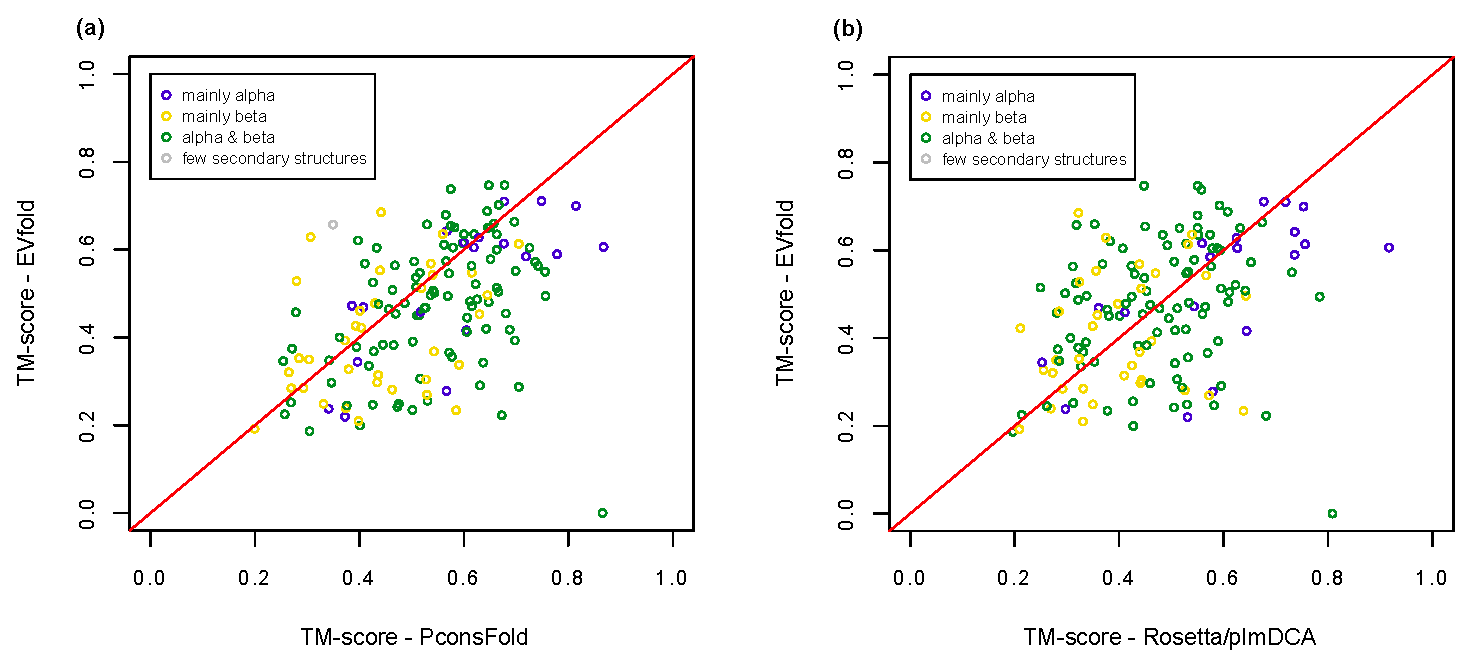
\includegraphics[scale=0.7]{figures/vs.eps}}
\caption{TM-score comparison for top-ranked models of the proteins in
 the PSICOV dataset. The decoys for each method were re-ranked using
 Pcons to assess the performance of the structure prediction process
 independent of the model ranking scheme. The colors represent all
 four CATH fold classes. (a) PconsFold compared to EVfold-PLM. (b)
 Rosetta/plmDCA compared to EVfold-PLM.}\label{fig:vs}
\end{figure*}

\subsection{PconsFold vs. EVfold }

When looking at Figure~\ref{fig:vs} the majority of alpha helical
proteins (blue) achieved higher TM-scores with PconsFold than with
EVfold-PLM. On average we see an improvement of 14\% of PconsFold over
EVfold-PLM on alpha helical proteins. The same improvement can also be
observed for Rosetta/plmDCA. Together with Figure~\ref{fig:main},
this indicates that Rosetta performs better on alpha-helical
proteins. The average
performance of PconsFold on alpha \& beta proteins (green) is 15\%
higher than for EVfold-PLM. However, Rosetta/plmDCA performs equally good
as EVfold-PLM on average on such targets. The improvement might thus be
due to PconsC contact maps, since it is only observable for PconsFold
and not for Rosetta/plmDCA. At a level of single proteins we see quite
some divergence between the results of EVfold-PLM and PconsFold in
Figure~\ref{fig:vs}. This is especially true for {\em mainly beta}
proteins and {\em alpha \& beta} proteins.

The analysis with MolProbity reveals that the backbone dihedral
quality of Rosetta models is higher than for EVfold-PLM models. The
percentage of Ramachandran outliers is 0.62\% for PconsFold and
12.16\% for EVfold-PLM. MolProbity further reports an average clash
score of 10.48 for PconsFold and 9.90 for EVfold-PLM. The EVfold-PLM
models have slightly less clashes than the models from PconsFold. The
average final MolProbity score is with 1.85 better for PconsFold then
2.38 for EVfold-PLM. This corresponds to a better average MolProbity
percentile rank of 80.69 for PconsFold than the average rank of 54.21
for EVfold-PLM.


Table~\ref{tab:evfold} contains TM-scores for the top-ranked models of
each protein in the small test dataset. We compare the EVfold results,
as published in \citeauthor{marks_protein_2011}
\citeyear{marks_protein_2011}, with results from the current EVfold-PLM
and PconsFold with 20,000 generated decoys. With an average TM-score of 0.55
EVfold-PLM performs 15\% better than EVfold with mean field,
showing the importance of improved contact prediction. When using
PconsFold there is an additional improvement of 16\% to an average
TM-score of 0.64. This further supports our observation that improved
contact maps improve structure prediction.


\begin{table}[!t]
\processtable{TM-scores for top ranked models comparing EVfold with
  mean field,  EVfold-PLM, and
 PconsFold with 20,000 decoys. \label{tab:evfold}}
{\begin{tabular}{lp{1.5cm}p{1.5cm}p{1.5cm}p{1.5cm}}\toprule
Protein & EVfold  & EVfold-PLM  & PconsFold\\\midrule
BPT1\_BOVIN & 0.49 & 0.25  & 0.57 \\
CADH1\_HUMAN & 0.55 & 0.54  & 0.53 \\
CD209\_HUMAN * & 0.39 & 0.64  & 0.54 \\
CHEY\_ECOLI & 0.65 & 0.66  & 0.82 \\
ELAV4\_HUMAN & 0.57 & 0.61  & 0.80 \\
O45418\_CAEEL & 0.48 & 0.62  & 0.65 \\
OMPR\_ECOLI & 0.35 & 0.44  & 0.59 \\
OPSD\_BOVIN & 0.50 & 0.55  & 0.56 \\
PCBP1\_HUMAN & 0.25 & 0.43  & 0.60 \\
RASH\_HUMAN & 0.70 & 0.62  & 0.67 \\
RNH\_ECOLI & 0.54 & 0.66  & 0.61 \\
SPTB2\_HUMAN & 0.37 & 0.51 & 0.74 \\
THIO\_ALIAC & 0.55 & 0.56  & 0.83 \\
TRY2\_RAT & 0.53 ** & 0.78  & 0.54 \\
YES\_HUMAN & 0.35 & 0.31  & 0.57 \\ \midrule
Mean & 0.48 & 0.55  & 0.64 \\ \botrule
\end{tabular}}{* The Uniprot entry A8MVQ9\_HUMAN of the EVfold publication was renamed into CD209\_HUMAN. ** This value was corrected as in the original publication it showed the value for the best possible model.}
\end{table}


\section{Conclusion}

Here, we show that improved contact predictions from PconsC
\cite[]{skwark_PconsC:_2013} actually lead to improvements in protein
structure prediction. Further, it is clear that for proteins with
better-predicted contacts the generated models are of higher quality,
i.e. future improvements in contact predictions will result in higher
quality models. A comparison between using Rosetta and CNS indicates
that using similar contact predictions generates models of similar
quality. However, Rosetta models are chemically more correct. Finally,
it is also clear that in many top ranked models the contacts are less
well satisfied than in the native structures, i.e. an improved folding
protocol would improve the models. One option would be to use
model-PPV as a measure of model quality, or as a stopping criterion
for decoy generation, another option is to use both CNS and Rosetta
and then try to identify the optimal model.



\section*{Acknowledgement}
Joel Hedlund is acknowledged for technical advice and valuable contributions to the code. 

\paragraph{Computational resources\textcolon}
The computations were performed on resources at PDC Centre for High
Performance Computing (PDC-HPC) and on resources provided by SNIC
through Uppsala Multidisciplinary Center for Advanced Computational
Science (UPPMAX) and National Supercomputer (NSC) Centre in Link\"oping,
Sweden.

\paragraph{Funding\textcolon} This work was supported by grants from
the Swedish Research Council (VR-NT 2012-5046, VR-M 2010-3555), SSF
(the Foundation for Strategic Research) and Vinnova through the
Vinnova-JSP program, and SeRC the Swedish E-science Research Center.
MJS is supported by the Academy of Finland Center of Excellence COIN.
DSM, CS and SH are supported by NIH award R01 GM106303.

\bibliographystyle{natbib}
%\bibliographystyle{achemnat}
%\bibliographystyle{plainnat}
%\bibliographystyle{abbrv}
%\bibliographystyle{bioinformatics}
%
%\bibliographystyle{plain}
%
\bibliography{pcons_fold}



\end{document}


